\documentclass{standalone}
\usepackage{tikz}

\begin{document}
 	\begin{tikzpicture}
 		\draw (5, 5) node {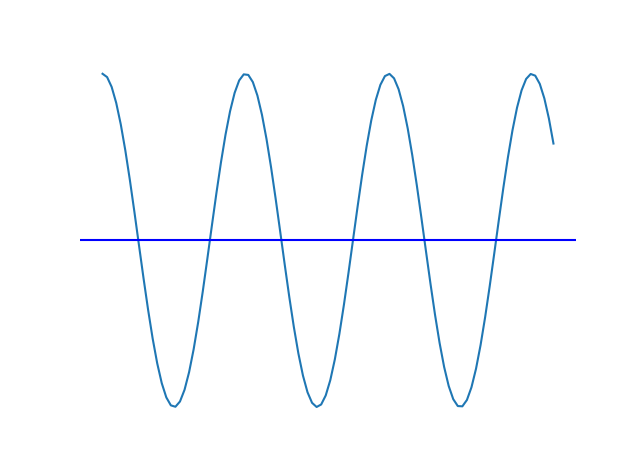
\includegraphics{../images/cosine_wave.png}};
 		%\draw[fill=black](0,0)--(5,0)--(5,5)--(5,0)--(0,0);
 		%\draw[ fill=black!20!white]  (0,0) grid (5,5) rectangle (0,0);
 		\draw[red, name=above,dashed]  (-0.6,9.1)--(4.9,0.7);
 		\draw[red, name=above,dashed] (10.4,9.1) --(4.9,0.7);
 		\draw[green, name=above,dashed] (-0.6,9.1)-- (1.2,0.7);
 		\draw[green, name=above,dashed] (10.4,9.1) --(4.9,0.7);
 		\draw[green, name=above,dashed] (10.4,9.1) --(4.9,0.7);
 		\draw[green, name=above,dashed] (10.4,9.1) --(4.9,0.7);
   		
 	\end{tikzpicture}
\end{document}